%%%%%%%%%%%%%%%%%%%%%%%%%%%%%%%%%%%%%%%%%%%%%%%%%%%%%%%%%%%%%%%%%%%%%%%%%%%%
\section{Supporting Information Appendix} \label{ap_c_vhgr}


\subsection{Simulated groundwater head for VHGR scenarios}

\begin{figure}[H]
\label{ap_c_heads}
  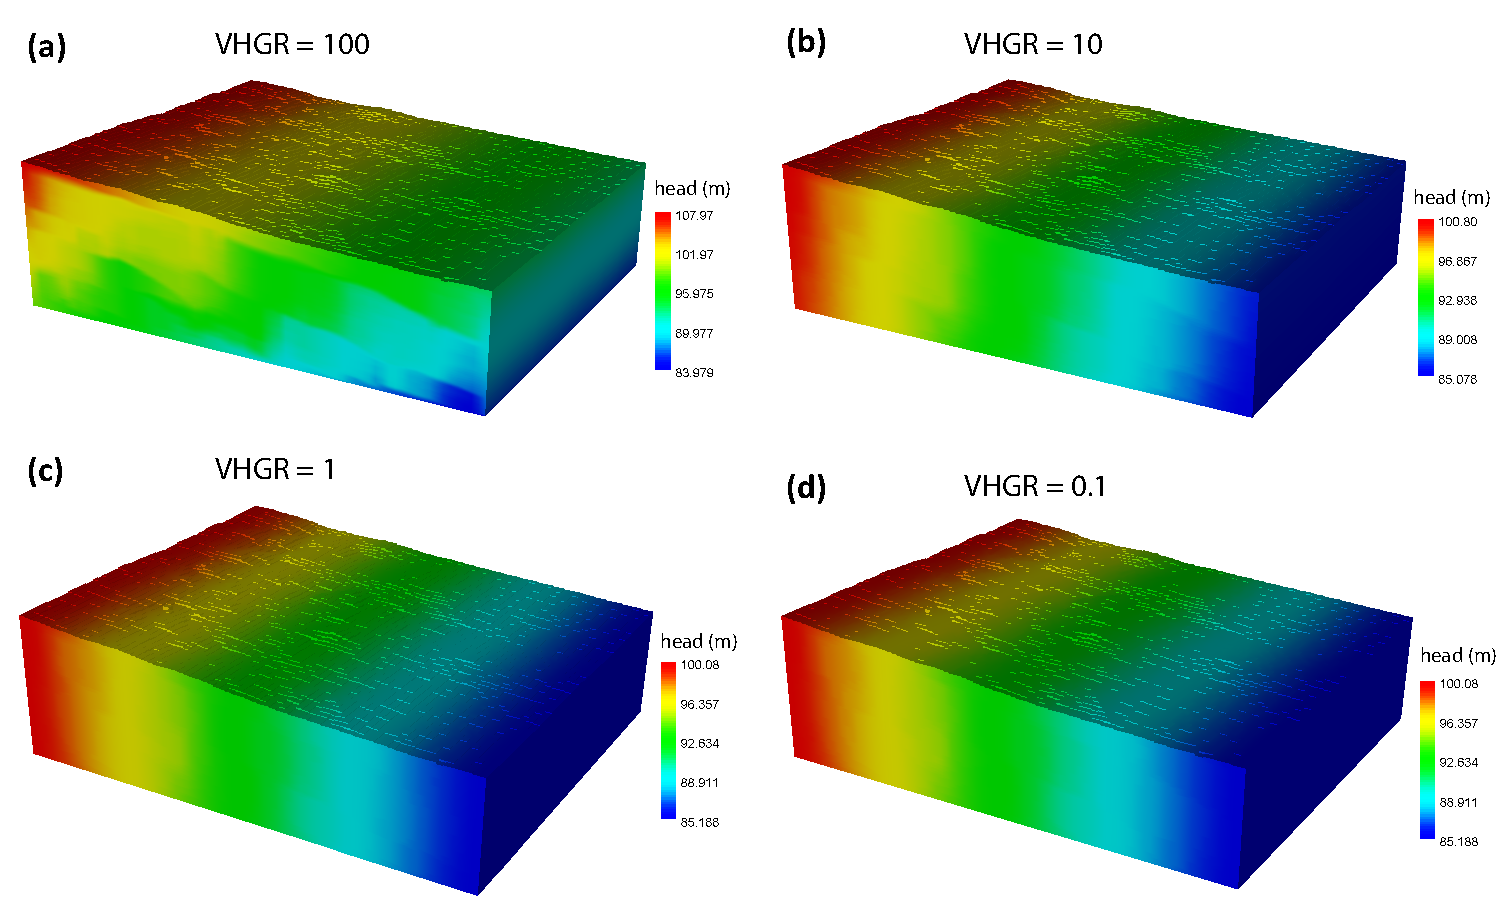
\includegraphics[width=\textwidth]{ch4_appendix_figs/heads.pdf}
  \caption{(a-d) Simulated steady state groundwater head across the 4 VHGR scenarios tested in this study.}
  \label{ap_c_heads_vhgr}
\end{figure}



%--------------------------------------------------------%
\subsection{Particle trajectory coordinate rotation and travel time normalization via the characteristic travel time}
\label{s_ap_c_part_rot}

In order to ensure comparability across the range of VHGR scenarios of differing travel times and mean flow direction, we perform coordinate rotations and normalize travel times by a characteristic travel time to travel the average facies length, $t_c$. 

First, we compute the mean Lagrangian velocity across all trajectories, $\bar{v}$ and use the characteristic time to travel the average facies length, $t_c$, to normalize time across VHGR scenarios (SI Appendix Table S1). The mean velocity and facies length are calculated along the direction of mean flow. Since this direction varies across VHGR, by an angle $\Phi$ relative to the horizontal direction, and the model outputs trajectories in a regular 3D Cartesian grid, we rotate the particle trajectory coordinates about the $x$ axis by $\Phi$ to recover the the transformed $y$ and $z$ components along the longitudinal and transverse vertical directions respectively ($y’$ and $z’$):

\begin{equation}
\begin{aligned}
\label{eq:rotation}
    y' = z \cdot sin(\Phi) + y \cdot cos(\Phi) \\
    z' = z \cdot cos(\Phi) - y \cdot sin(\Phi)
\end{aligned}
\end{equation}

Flow occurs along $zy$, thus the $x$ coordinates (transverse horizontal) remain unchanged. After transforming coordinates according to (\ref{eq:rotation}), we calculate longitudinal displacement along $y’$, transverse vertical displacement along $z’$, and transverse horizontal displacement along $x$.



\bgroup

\renewcommand{\arraystretch}{1.5}

\setlength{\tabcolsep}{20pt}

\begin{table}[H]

\caption{Mean velocity $\bar{v}$ along the longitudinal direction ($y'$), the angle of mean flow, relative to the horizontal direction in the un-rotated Cartesian coordinate system $\Phi$, the characteristic hydrofacies length $\lamdba_c$ along the longitudinal direction, and the characteristic time $t_c$ along the longitudinal direction ($t_c = l_c / \bar{v}$).} 
\centering


\begin{tabular}{lrrrr}
\label{ap_c_tc}

\textbf{VHGR} & $\bm{\Phi} (^{\circ})$ & $\bm{l_c \: \: (m)}$ & $\bm{\bar{v} \: \: (m/yr)}$ & $\bm{t_c \: \: (yr)}$  \\ 
\hline
   100 & 89.43 & 2.19  & 73.33 & 0.046 \\
   10  & 84.29 & 2.20  & 8.40  & 0.252 \\
   1   & 45.00 & 3.09  & 7.20  & 0.093 \\
   0.1 & 5.71  & 21.97 & 53.01 & 0.319 \\
\hline
\end{tabular}

\end{table}
\egroup




%--------------------------------------------------------%
\subsection{RW3D parameters}


% 01_mm_plots_tables.R in F:/ ... POst_QE_Research/DISSERTATION/01_mm
% search for gw_and_sw_c_summary table


\bgroup

\renewcommand{\arraystretch}{1.5}

\setlength{\tabcolsep}{20pt}

\begin{table}[H]

\caption{RW3D parameters for each VHGR scenario including the number of injected particles (particle count), the maximum simulation time (max time), and the number of snapshots saved (snapshot count). Note that the snapshot count = max time $\cdot$ 10 000, meaning that for each scenario, 100 snapshots were taken per year of simulation time.} 
\centering

\begin{tabular}{lrrr}
\label{ap_c_rw3d_params}

\textbf{VHGR} & \textbf{particle count} & \textbf{max time (yrs)} & \textbf{snapshot count}  \\ 
\hline
   100 & 10 000  & 100   & 10 000  \\
   10  & 10 000  & 500   & 50 000  \\
   1   & 10 000  & 1000 & 100 000 \\
   0.1 & 10 000  & 5000 & 500 000 \\
\hline
\end{tabular}

\end{table}
\egroup








%--------------------------------------------------------%
\subsection{Hydrofacies proportions over time}



\begin{figure}[H]
  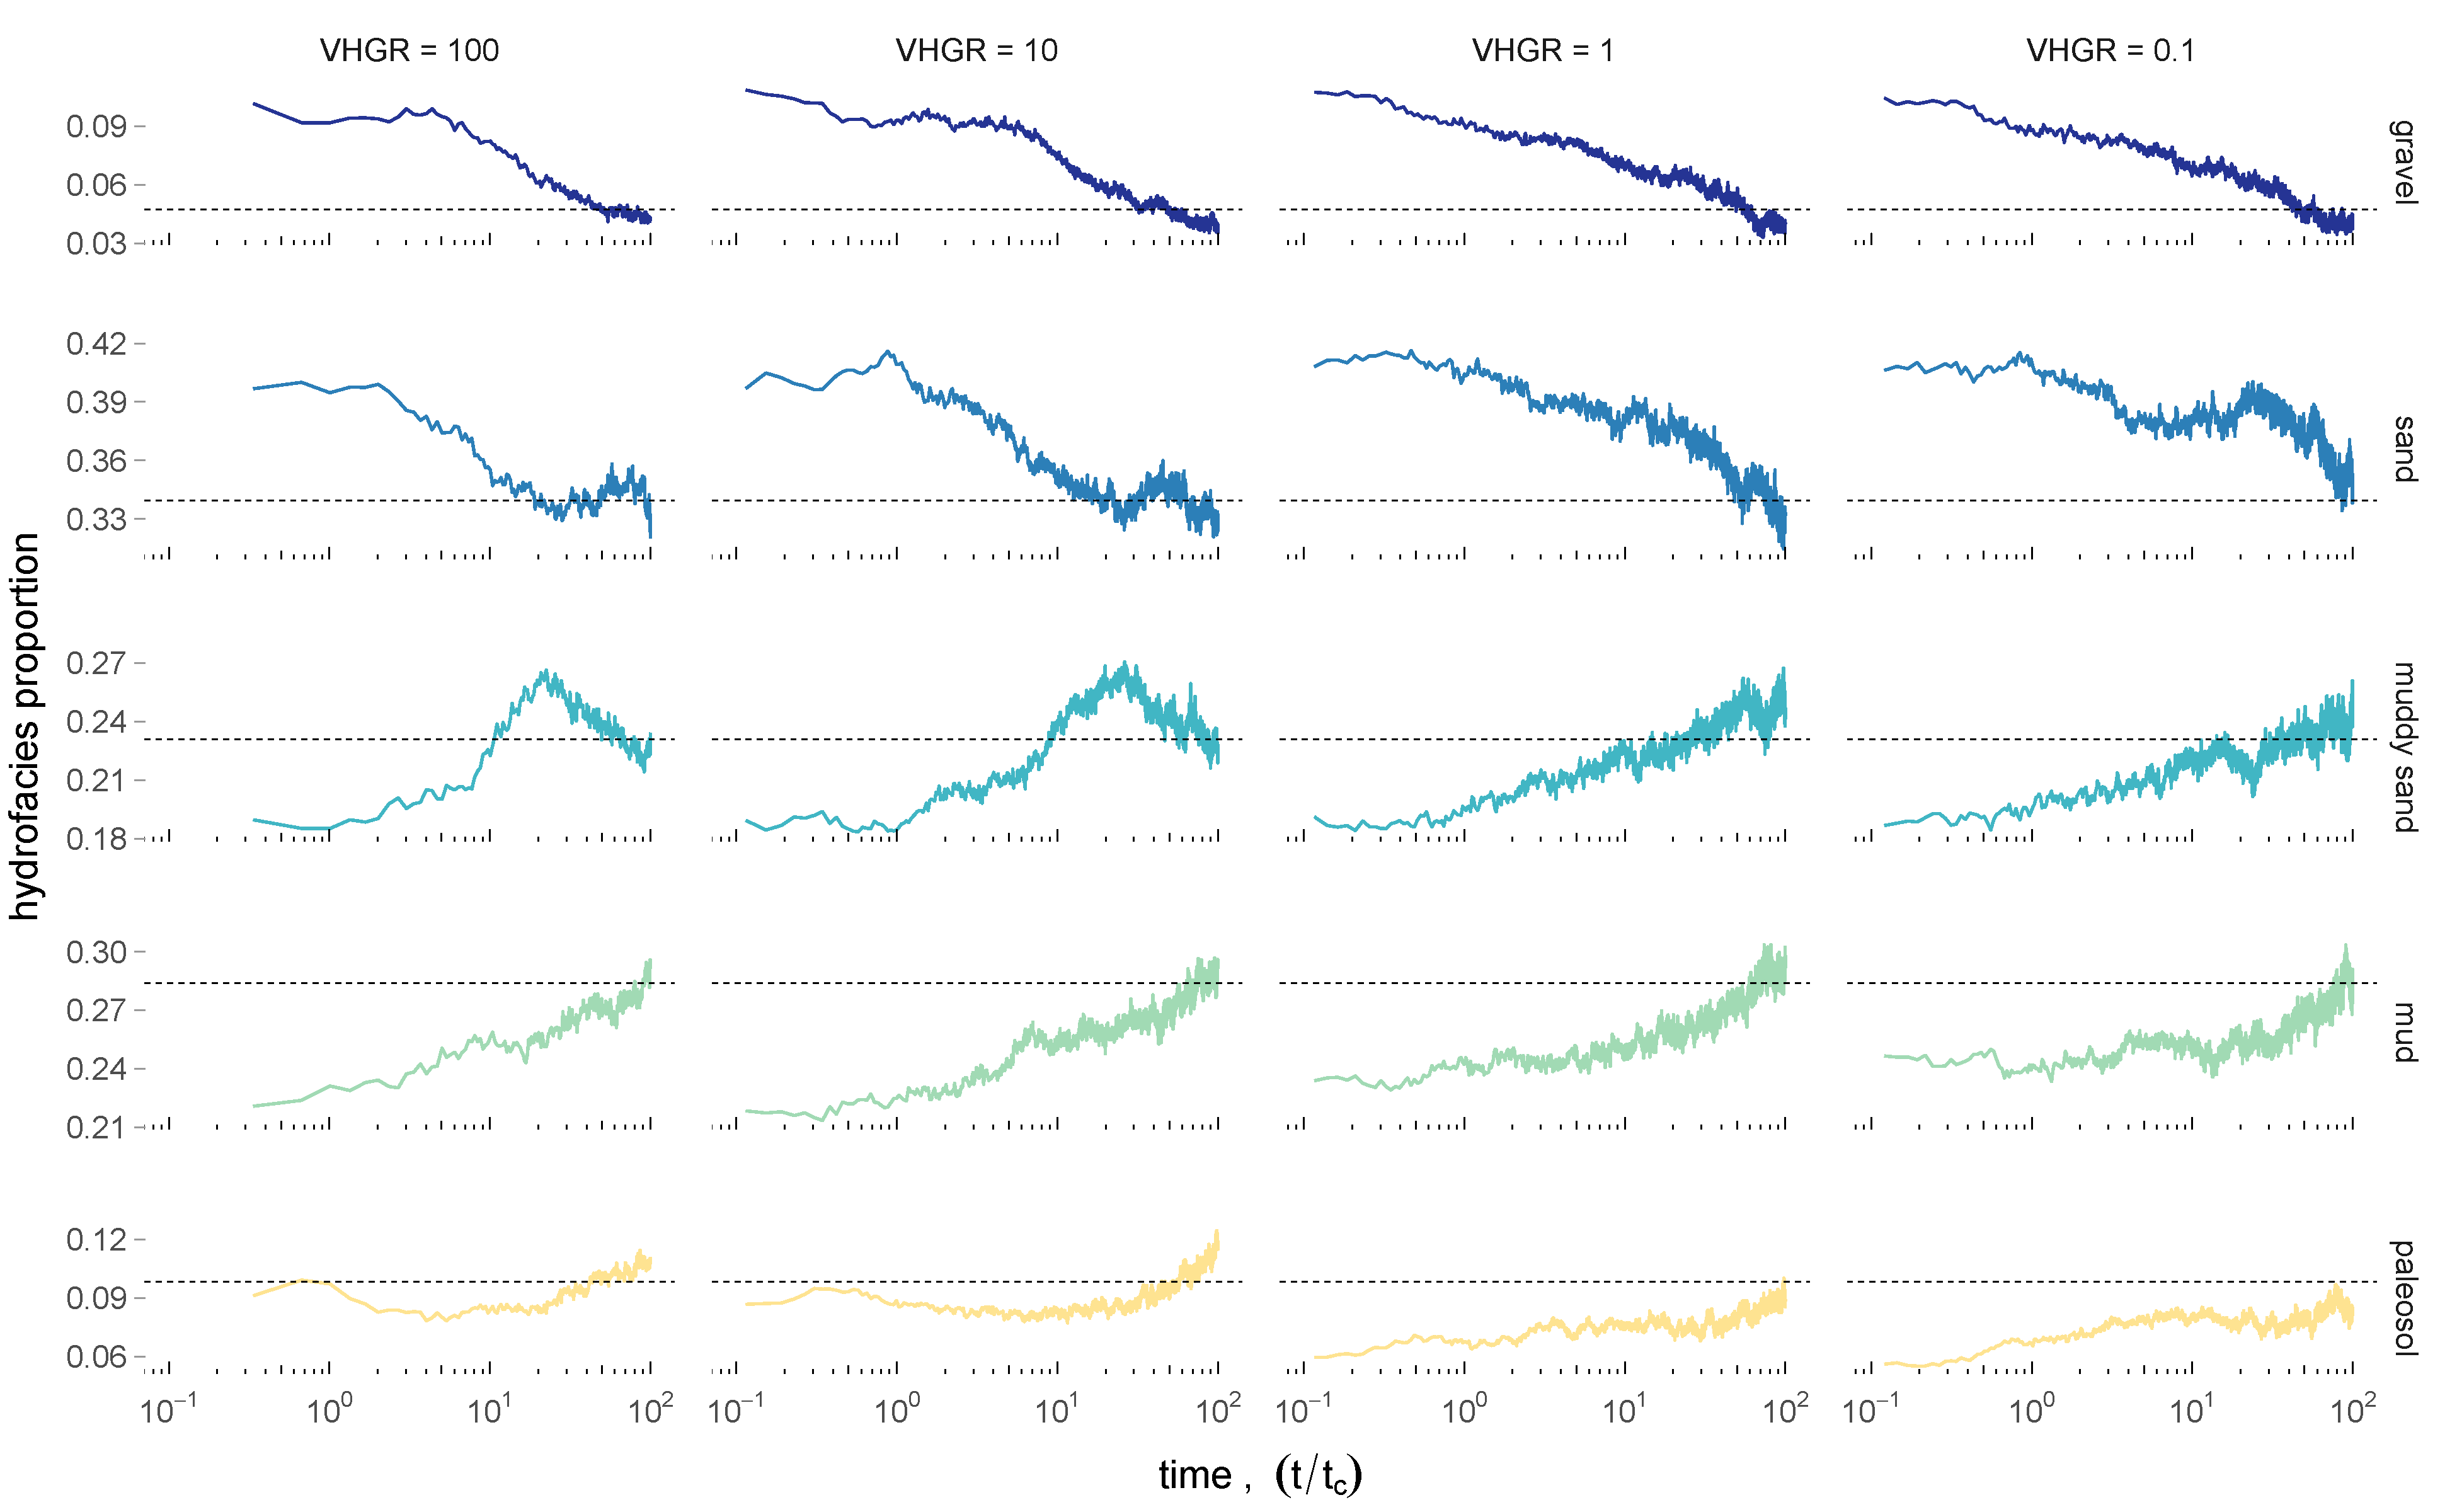
\includegraphics[width=\textwidth]{ch4_appendix_figs/phf_over_time_00_03_ai.pdf}
  \caption{Proportion of hydrofacies occupied by the particles as a function of time across the 4 VHGR scenarios indicate mixing: over about 32 characteristic times, proportions converge onto the hydrofacies proportions shown as black, dashed horizontal lines. Note the difference in y axis between the rows, each of which correspond to a distinct hydrofacies..}
  \label{ap_c_heads_vhgr}
\end{figure}



\clearpage



%--------------------------------------------------------%
% Acknowledgments
%--------------------------------------------------------%
\section{Acknowledgments}

We gratefully thank Drs. Yong Zhang, Marco Dentz, and Song Wei for their feedback and modeling advice. Support for this research was provided by the National Science Foundation (NSF) Climate Change, Water, and Society (CCWAS) Integrated Graduate Education and Research Traineeship (IGERT) program at the University of California, Davis (http://ccwas.ucdavis.edu, DGE-10693333), and by the U.S./China Clean Energy Research Center for Water-Energy Technologies (CERC-WET). %All data is accessible via Dryad at \textit{URL WITH DOI TO BE INPUT}, and procedures and models are accessible via Github at \textit{URL WITH DOI TO BE INPUT}.  




\clearpage